\documentclass[12pt]{article}  % 确定normalsize大小,为可选参数,在中括号内,此为10磅,只有10,11,12磅三个选项
\usepackage{ctex}

\newcommand{\myfont}{\textit{\textbf{\textsf{Fancy Text}}}} % 自定义字体
\usepackage[colorlinks,linkcolor=red]{hyperref}

\usepackage{geometry}
\usepackage{graphicx}
\usepackage{pythonhighlight}
\usepackage{listings}
\usepackage{float}
\usepackage{xcolor}
\usepackage{pgfplots}
% 定义页边距
\geometry{left=1.5cm,right=1.5cm,top=2.0cm,bottom=2.0cm}
% 定义可能使用到的颜色
\definecolor{CPPLight}  {HTML} {686868}
\definecolor{CPPSteel}  {HTML} {888888}
\definecolor{CPPDark}   {HTML} {262626}
\definecolor{CPPBlue}   {HTML} {4172A3}
\definecolor{CPPGreen}  {HTML} {487818}
\definecolor{CPPBrown}  {HTML} {A07040}
\definecolor{CPPRed}    {HTML} {AD4D3A}
\definecolor{CPPViolet} {HTML} {7040A0}
\definecolor{CPPGray}  {HTML} {B8B8B8}
\lstset{
    columns=fixed,
    numbers=left,                                      			% 在左侧显示行号
    frame=single,                                          	% 不显示背景边框
    backgroundcolor=\color[RGB]{245,245,244},            		% 设定背景颜色
    keywordstyle=\color[RGB]{40,40,255},                		% 设定关键字颜色
    numberstyle=\footnotesize\color{darkgray},         			% 设定行号格式
    commentstyle=\it\color[RGB]{0,96,96},               	  % 设置代码注释的格式
    stringstyle=\rmfamily\slshape\color[RGB]{128,0,0},   		% 设置字符串格式
    showstringspaces=false,                            			% 不显示字符串中的空格
    language=c++,                                       		% 设置语言
    morekeywords={alignas,continute,friend,register,true,alignof,decltype,goto,
    reinterpret_cast,try,asm,defult,if,return,typedef,auto,delete,inline,short,
    typeid,bool,do,int,signed,typename,break,double,long,sizeof,union,case,
    dynamic_cast,mutable,static,unsigned,catch,else,namespace,static_assert,using,
    char,enum,new,static_cast,virtual,char16_t,char32_t,explict,noexcept,struct,
    void,export,nullptr,switch,volatile,class,extern,operator,template,wchar_t,
    const,false,private,this,while,constexpr,float,protected,thread_local,
    const_cast,for,public,throw,std},
    emph={map,set,multimap,multiset,unordered_map,unordered_set,
    unordered_multiset,unordered_multimap,vector,string,list,deque,
    array,stack,forwared_list,iostream,memory,shared_ptr,unique_ptr,
    random,bitset,ostream,istream,cout,cin,endl,move,default_random_engine,
    uniform_int_distribution,iterator,algorithm,functional,bing,numeric,},
    emphstyle=\color{CPPViolet},
}

\author{Anonymous}
\title{\Huge ComputerNote}
\date{}

\begin{document} % 文稿区

\maketitle

\renewcommand{\contentsname}{\large Contents}
\tableofcontents

\section{算法}

\subsection{Disjoint Set Union(并查集:DSU算法)}

并查集,在一些有N个元素的集合应用问题中,我们通常是在开始时让每个元素构成一个单元素的集合,然后按一定顺序将属于同一组的元素所在的集合合并,其间要反复查找一个元素在哪个集合中。

使用并查集时,首先会存在一组不相交的动态集合 $S = \left\{ {{S_1},{S_2}, \cdots ,{S_k}} \right\}$,一般都会使用一个整数表示集合中的一个元素。

每个集合可能包含一个或多个元素,并选出集合中的某个元素作为代表。每个集合中具体包含了哪些元素是不关心的,具体选择哪个元素作为代表一般也是不关心的。我们关心的是,对于给定的元素,可以很快的找到这个元素所在的集合(的代表),以及合并两个元素所在的集合,而且这些操作的时间复杂度都是常数级的。

并查集的基本操作有三个:

makeSet(s):建立一个新的并查集,其中包含 s 个单元素集合。

unionSet(x, y):把元素 x 和元素 y 所在的集合合并,要求 x 和 y 所在的集合不相交,如果相交则不合并。

find(x):找到元素 x 所在的集合的代表,该操作也可以用于判断两个元素是否位于同一个集合,只要将它们各自的代表比较一下就可以了。

并查集的实现原理也比较简单,就是使用树来表示集合,树的每个节点就表示集合中的一个元素,树根对应的元素就是该集合的代表,如图 1-1-1 所示。

\begin{figure}[h]
\centering
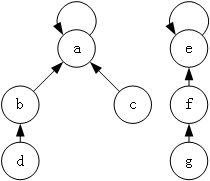
\includegraphics[width = 6cm ]{1-1-1.png}

图 1-1-1 并查集的树表示
\end{figure}

图中有两棵树,分别对应两个集合,其中第一个集合为 $\left\{ a, b, c, d \right\}$,代表元素是 $a$;第二个集合为 $\left\{ e, f, g \right\}$,代表元素是 $e$。

树的节点表示集合中的元素,指针表示指向父节点的指针,根节点的指针指向自己,表示其没有父节点。沿着每个节点的父节点不断向上查找,最终就可以找到该树的根节点,即该集合的代表元素。

现在,应该可以很容易的写出 makeSet 和 find 的代码了,假设使用一个足够长的数组来存储树节点(很类似之前讲到的静态链表),那么 makeSet 要做的就是构造出如图 2 的森林,其中每个元素都是一个单元素集合,即父节点是其自身:

\begin{figure}[h]
\centering
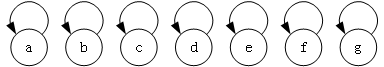
\includegraphics[width = 10cm ]{1-1-2.png}

图 1-1-2 构造并查集初始化
\end{figure}

接下来,就是 find 操作了,如果每次都沿着父节点向上查找,那时间复杂度就是树的高度,完全不可能达到常数级。这里需要应用一种非常简单而有效的策略——路径压缩。

路径压缩,就是在每次查找时,令查找路径上的每个节点都直接指向根节点,如图 1-1-3 所示。

\begin{figure}[h]
\centering
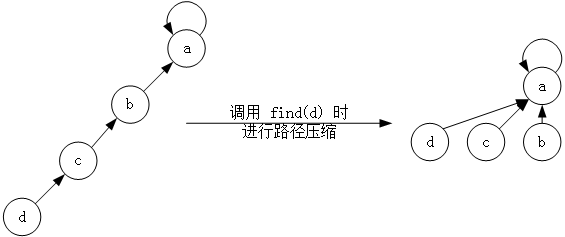
\includegraphics[width = 10cm ]{1-1-3.png}

图 1-1-3 路径压缩
\end{figure}

最后是合并操作 unionSet,并查集的合并也非常简单,就是将一个集合的树根指向另一个集合的树根,如图 1-1-4 所示。

\begin{figure}[h]
\centering
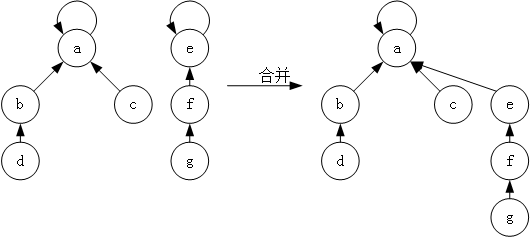
\includegraphics[width = 10cm ]{1-1-4.png}

图 1-1-4 并查集的合并
\end{figure}

这里也可以应用一个简单的启发式策略——按秩合并。该方法使用秩来表示树高度的上界,在合并时,总是将具有较小秩的树根指向具有较大秩的树根。简单的说,就是总是将比较矮的树作为子树,添加到较高的树中。为了保存秩,需要额外使用一个与 uset 同长度的数组,并将所有元素都初始化为 0。

除了按秩合并,并查集还有一种常见的策略,就是按集合中包含的元素个数(或者说树中的节点数)合并,将包含节点较少的树根,指向包含节点较多的树根。这个策略与按秩合并的策略类似,同样可以提升并查集的运行速度,而且省去了额外的 rank 数组。

并查集的空间复杂度是 $O(n)$ 的,这个很显然,如果是按秩合并的,占的空间要多一些。find 和 unionSet 操作都可以看成是常数级的,或者准确来说,在一个包含 $n$ 个元素的并查集中,进行 $m$ 次查找或合并操作,最坏情况下所需的时间为 $O\left( {m \alpha (n)} \right)$,这里的 $\alpha$ 是 Ackerman 函数的某个反函数,在极大的范围内(比可观察到的宇宙中估计的原子数量 $10^{80}$ 还大很多)都可以认为是不大于 4 的。

\textbf{Description:}

若某个家族人员过于庞大,要判断两个是否是亲戚,确实还很不容易,给出某个亲戚关系图,求任意给出的两个人是否具有亲戚关系。 规定:x和y是亲戚,y和z是亲戚,那么x和z也是亲戚。如果x,y是亲戚,那么x的亲戚都是y的亲戚,y的亲戚也都是x的亲戚。

\textbf{Input:}

第一行:三个整数n,m,p,($n \le 5000,m \le 5000,p \le 5000$),分别表示有n个人,m个亲戚关系,询问p对亲戚关系。 以下m行:每行两个数$M_i,M_j$,$1 \le M_i,M_j \le N$,表示$M_i和M_j$具有亲戚关系。 接下来p行:每行两个数$P_i,P_j,$询问$P_i$和$P_j$是否具有亲戚关系。

\textbf{Output:}

P行,每行一个’Yes’或’No’。表示第i个询问的答案为“具有”或“不具有”亲戚关系。

\subsection{Meet-in-the-middle(split and merge)}

Meet in the middle(有时候也叫作split and merge)是一种用以获取足够高效解决方案的灵巧的思想。和分治思想非常类似,它将问题分割成两个部分,然后试着合并这两个子问题的结果。好处在于通过使用一点额外的空间,你可以解决两倍规模的原来可以解决的问题。

\textbf{4和问题(流行的面试问题)}

给定一个整数数组A,问数组中是否存在4个数,使得这4个数的和是0(同一个元素可以被多次使用)。例如:数组A = [2, 3, 1, 0, -4, -1],一种可能的方案是3 + 1 + 0 - 4 = 0 或 0 + 0 + 0 + 0 = 0。

朴素的算法是判断所有可能的4个数的组合,这种方案需要计算$O(N^4)$次。

一个些微改进的算法是暴力搜索所有的可能的$n^3$个3个数的组合,并且用hash表来判断-(a+b+c)是否在原始的数组中。这个算法的复杂度是$O(n^3)$到目前为止,你可能想知道meet in the middle在这里要怎么应用,最关键的洞察来自于改写$a + b + c + d = 0$成$a + b = -(c + d)$。现在我们可以存储$n^2$个a+b的和在一个hash表S中,然后可以枚举所有可能c和d的$n^2$种组合并且判断S中是否包括-(c+d)。

 这个算法的时间复杂度和空间复杂度都是$O(n^2)$,这个问题没有已知的更快的算法

\textbf{双向搜索}

\subsection{字符串匹配算法}

\subsubsection{KMP}

\subsection{排序算法}

\subsubsection{快速排序}

\subsubsection{拓扑排序}

定义:将有向图中的顶点以线性方式进行排序。即对于任何连接自顶点u到顶点v的有向边uv,在最后的排序结果中,顶点u总是在顶点v的前面。

一个有向图能被拓扑排序的充要条件就是它是一个有向无环图(DAG:Directed Acyclic Graph)。


复杂度分析:
复杂度同DFS一致,即O(E+V)。具体而言,首先需要保证图是有向无环图,判断图是DAG可以使用基于DFS的算法,复杂度为O(E+V),而后面的拓扑排序也是依赖于DFS,复杂度为O(E+V)

\subsection{动态规划}

\subsection{贪心算法}

\subsection{Dancing Linker}

\url{https://www.jianshu.com/p/93b52c37cc65}

\section{数据结构}

\subsection{链表}

\subsection{队列}

\subsection{栈}

\subsection{树}

\subsubsection{B-Tree}

\subsubsection{AVL Tree}

\subsubsection{Red-Black Tree}

\subsubsection{VEb Tree}

\subsubsection{Spanning Tree}

Spanning Tree:

In the mathematical field of graph theory, a spanning tree T of an undirected graph G is a subgraph that is a tree which includes all of the vertices of G, with minimum possible number of edges. In general, a graph may have several spanning trees, but a graph that is not connected will not contain a spanning tree (but see Spanning forests below). If all of the edges of G are also edges of a spanning tree T of G, then G is a tree and is identical to T (that is, a tree has a unique spanning tree and it is itself).

Minium Spanning Tree:

A minimum spanning tree (MST) or minimum weight spanning tree is a subset of the edges of a connected, edge-weighted (un)directed graph that connects all the vertices together, without any cycles and with the minimum possible total edge weight. That is, it is a spanning tree whose sum of edge weights is as small as possible. More generally, any edge-weighted undirected graph (not necessarily connected) has a minimum spanning forest, which is a union of the minimum spanning trees for its connected components.

\subsection{图}

\subsection{堆}

\subsection{散列表}

\section{编程语言}

\subsection{C/C++}

\subsubsection{内存分配}

\subsubsection{STL}

\subsection{JAVA}

\subsection{Python}

\subsubsection{装饰器}

\section{例题}

\subsection{求数组的最大子序列和}

给定整数$A_1,A_2,\ldots,A_N$(可能有负数),求$\sum_{k=i}^jA_k$的最大值(为方便起见,如果所有的整数均为负数,则最大子序列和为0。

代码如下,时间复杂度为\emph{O}(\emph{N})。
{\setmainfont{Menlo}
\begin{lstlisting}
int MaxSubsequenceSum(const int A[], int N) {
    int ThisSum, MaxSum, j;
    ThisSum = MaxSum = 0;
    for (j = 0; j < N; j++) {
        ThisSum += A[j];
        if (ThisSum > MaxSum) {
            MaxSum = ThisSum;
        } else if (ThisSum < 0) {
            ThisSum = 0;
        }
    }
    return MaxSum;
}
\end{lstlisting}}

\subsection{Binary Search}

给定一个整数X和整数$A_0,A_1,\ldots,A_{N-1},$后者已经预选排序好,求使得$A_i = X$的下标i,
如果X不在数据中,则返回i = -1。

\subsection{A + B}

Write a function that add two numbers A and B. You should not use + or any arithmetic operators.

Code:
{\setmainfont{Menlo}
\begin{lstlisting}
int aplusb(int a, int b) {
    // 主要利用异或运算来完成
    // 异或运算有一个别名叫做:不进位加法
    // 那么a ^ b就是a和b相加之后,该进位的地方不进位的结果
    // 然后下面考虑哪些地方要进位,自然是a和b里都是1的地方
    // a & b就是a和b里都是1的那些位置,a & b << 1 就是进位
    // 之后的结果。所以:a + b = (a ^ b) + (a & b << 1)
    // 令a' = a ^ b, b' = (a & b) << 1
    // 可以知道,这个过程是在模拟加法的运算过程,进位不可能
    // 一直持续,所以b最终会变为0。因此重复做上述操作就可以
    // 求得a + b的值。
    while (b != 0) {
        int _a = a ^b;
        int _b = (a & b) << 1;
        a = _a;
        b = _b;
    }
    return a;
}
\end{lstlisting}}

\subsection{Trailing Zeros}

Write an algorithm which computes the number of trailing zeros in n factorial.

Code:
{\setmainfont{Menlo}
\begin{lstlisting}
long long trailingZeros(long long n) {
    long long anw = 0;
    while (n >= 5) {
        anw += n / 5;
        n = n / 5;
    }
    return anw;
}
\end{lstlisting}}

\subsection{ugly number \uppercase\expandafter{\romannumeral2}}

Ugly number is a number that only have factors 2, 3 and 5.

Design an algorithm to find the nth ugly number. The first 10 ugly numbers are 1, 2, 3, 4, 5, 6, 8, 9, 10, 12...

O(nlogn) or O(n) time.

Notice:

Note that 1 is typically treated as an ugly number.

{\setmainfont{Menlo}
\begin{lstlisting}
#define min(a, b) ((a) < (b)? (a):(b))
#define min3(a, b, c) (min(min(a, b),min(a, c)))
int nthUglyNumber(int n) {
    // write your code here
    int i = 1;
    int p2 = 0;
    int p3 = 0;
    int p5 = 0;
    int uglyNum[6048] = {0};
    uglyNum[0] = 1;
    while (i < n) {
        uglyNum[i] = min3(uglyNum[p2] * 2, uglyNum[p3] * 3, uglyNum[p5] * 5);
        if (uglyNum[i] == uglyNum[p2] * 2) {
            p2++;
        }
        if (uglyNum[i] == uglyNum[p3] * 3) {
            p3++;
        }
        if (uglyNum[i] == uglyNum[p5] * 5) {
            p5++;
        }
        i++;
    }
    return uglyNum[n - 1];
}
\end{lstlisting}}

\section{其他}

\subsection{位移运算}

\paragraph{位移运算}

\begin{table}[h]
   \centering
   \begin{tabular}{|l|c|c|}             \hline
     符号 & 描述 & 运算规则               \\\hline
     \&       & 与     & 两个位都为1时,结果才为1    \\
     |        & 或     & 两个位都为0时,结果才为0                      \\
     $\wedge$ & 异或    & 两个位相同为0,相异为1                      \\
     $\sim$   & 取反    & 0变1,1变0                      \\
     $\ll$    & 左移    & 各二进位全部左移若干位,高位丢弃,低位补0                     \\
     $\gg$    & 右移    & 各二进位全部右移若干位,对无符号数,高位补0,有符号数,\\
     &&各编译器处理方法不一样,\\
     &&有的补符号位(算术右移),有的补0(逻辑右移)                     \\\hline
   \end{tabular}
   \caption{常见位移运算}
   \label{tab:Margin_settings}
\end{table}

注意以下几点:

1.  在这6种操作符,只有$\sim$取反是单目操作符,其它5种都是双目操作符。

2.  位操作只能用于整形数据,对float和double类型进行位操作会被编译器报错。

3.  对于移位操作,在微软的VC6.0和VS2008编译器都是采取算术称位即算术移位操作,算术移位是相对于逻辑移位,它们在左移操作中都一样,低位补0即可,但在右移中逻辑移位的高位补0而算术移位的高位是补符号位。

4.  位操作符的运算优先级比较低,因为尽量使用括号来确保运算顺序,否则很可能会得到莫明其妙的结果。比如要得到像1,3,5,9这些$2^i+1$的数字。写成int a = 1 << i + 1;是不对的,程序会先执行i + 1,再执行左移操作。应该写成int a = (1 << i) + 1;

5.  另外位操作还有一些复合操作符,如\&=、|=、 $\wedge$=、<<=、>>=。

\paragraph{位移运算技巧}

\subparagraph{判断奇偶}
只要根据最未位是0还是1来决定,为0就是偶数,为1就是奇数。因此可以用if ((a \& 1) == 0)代替if (a \% 2 == 0)来判断a是不是偶数。

\subparagraph{交换两数}
交换a和b
{\setmainfont{Menlo}
\begin{lstlisting}
void Swap(int &a, int &b){
  if (a != b){
    a ^= b;
    b ^= a;
    a ^= b;
  }
}
\end{lstlisting}}


\end{document}
